\documentclass[1p]{elsarticle_modified}
%\bibliographystyle{elsarticle-num}

%\usepackage[colorlinks]{hyperref}
%\usepackage{abbrmath_seonhwa} %\Abb, \Ascr, \Acal ,\Abf, \Afrak
\usepackage{amsfonts}
\usepackage{amssymb}
\usepackage{amsmath}
\usepackage{amsthm}
\usepackage{scalefnt}
\usepackage{amsbsy}
\usepackage{kotex}
\usepackage{caption}
\usepackage{subfig}
\usepackage{color}
\usepackage{graphicx}
\usepackage{xcolor} %% white, black, red, green, blue, cyan, magenta, yellow
\usepackage{float}
\usepackage{setspace}
\usepackage{hyperref}

\usepackage{tikz}
\usetikzlibrary{arrows}

\usepackage{multirow}
\usepackage{array} % fixed length table
\usepackage{hhline}

%%%%%%%%%%%%%%%%%%%%%
\makeatletter
\renewcommand*\env@matrix[1][\arraystretch]{%
	\edef\arraystretch{#1}%
	\hskip -\arraycolsep
	\let\@ifnextchar\new@ifnextchar
	\array{*\c@MaxMatrixCols c}}
\makeatother %https://tex.stackexchange.com/questions/14071/how-can-i-increase-the-line-spacing-in-a-matrix
%%%%%%%%%%%%%%%

\usepackage[normalem]{ulem}

\newcommand{\msout}[1]{\ifmmode\text{\sout{\ensuremath{#1}}}\else\sout{#1}\fi}
%SOURCE: \msout is \stkout macro in https://tex.stackexchange.com/questions/20609/strikeout-in-math-mode

\newcommand{\cancel}[1]{
	\ifmmode
	{\color{red}\msout{#1}}
	\else
	{\color{red}\sout{#1}}
	\fi
}

\newcommand{\add}[1]{
	{\color{blue}\uwave{#1}}
}

\newcommand{\replace}[2]{
	\ifmmode
	{\color{red}\msout{#1}}{\color{blue}\uwave{#2}}
	\else
	{\color{red}\sout{#1}}{\color{blue}\uwave{#2}}
	\fi
}

\newcommand{\Sol}{\mathcal{S}} %segment
\newcommand{\D}{D} %diagram
\newcommand{\A}{\mathcal{A}} %arc


%%%%%%%%%%%%%%%%%%%%%%%%%%%%%5 test

\def\sl{\operatorname{\textup{SL}}(2,\Cbb)}
\def\psl{\operatorname{\textup{PSL}}(2,\Cbb)}
\def\quan{\mkern 1mu \triangleright \mkern 1mu}

\theoremstyle{definition}
\newtheorem{thm}{Theorem}[section]
\newtheorem{prop}[thm]{Proposition}
\newtheorem{lem}[thm]{Lemma}
\newtheorem{ques}[thm]{Question}
\newtheorem{cor}[thm]{Corollary}
\newtheorem{defn}[thm]{Definition}
\newtheorem{exam}[thm]{Example}
\newtheorem{rmk}[thm]{Remark}
\newtheorem{alg}[thm]{Algorithm}

\newcommand{\I}{\sqrt{-1}}
\begin{document}

%\begin{frontmatter}
%
%\title{Boundary parabolic representations of knots up to 8 crossings}
%
%%% Group authors per affiliation:
%\author{Yunhi Cho} 
%\address{Department of Mathematics, University of Seoul, Seoul, Korea}
%\ead{yhcho@uos.ac.kr}
%
%
%\author{Seonhwa Kim} %\fnref{s_kim}}
%\address{Center for Geometry and Physics, Institute for Basic Science, Pohang, 37673, Korea}
%\ead{ryeona17@ibs.re.kr}
%
%\author{Hyuk Kim}
%\address{Department of Mathematical Sciences, Seoul National University, Seoul 08826, Korea}
%\ead{hyukkim@snu.ac.kr}
%
%\author{Seokbeom Yoon}
%\address{Department of Mathematical Sciences, Seoul National University, Seoul, 08826,  Korea}
%\ead{sbyoon15@snu.ac.kr}
%
%\begin{abstract}
%We find all boundary parabolic representation of knots up to 8 crossings.
%
%\end{abstract}
%\begin{keyword}
%    \MSC[2010] 57M25 
%\end{keyword}
%
%\end{frontmatter}

%\linenumbers
%\tableofcontents
%
\newcommand\colored[1]{\textcolor{white}{\rule[-0.35ex]{0.8em}{1.4ex}}\kern-0.8em\color{red} #1}%
%\newcommand\colored[1]{\textcolor{white}{ #1}\kern-2.17ex	\textcolor{white}{ #1}\kern-1.81ex	\textcolor{white}{ #1}\kern-2.15ex\color{red}#1	}

{\Large $\underline{11a_{87}~(K11a_{87})}$}

\setlength{\tabcolsep}{10pt}
\renewcommand{\arraystretch}{1.6}
\vspace{1cm}\begin{tabular}{m{100pt}>{\centering\arraybackslash}m{274pt}}
\multirow{5}{120pt}{
	\centering
	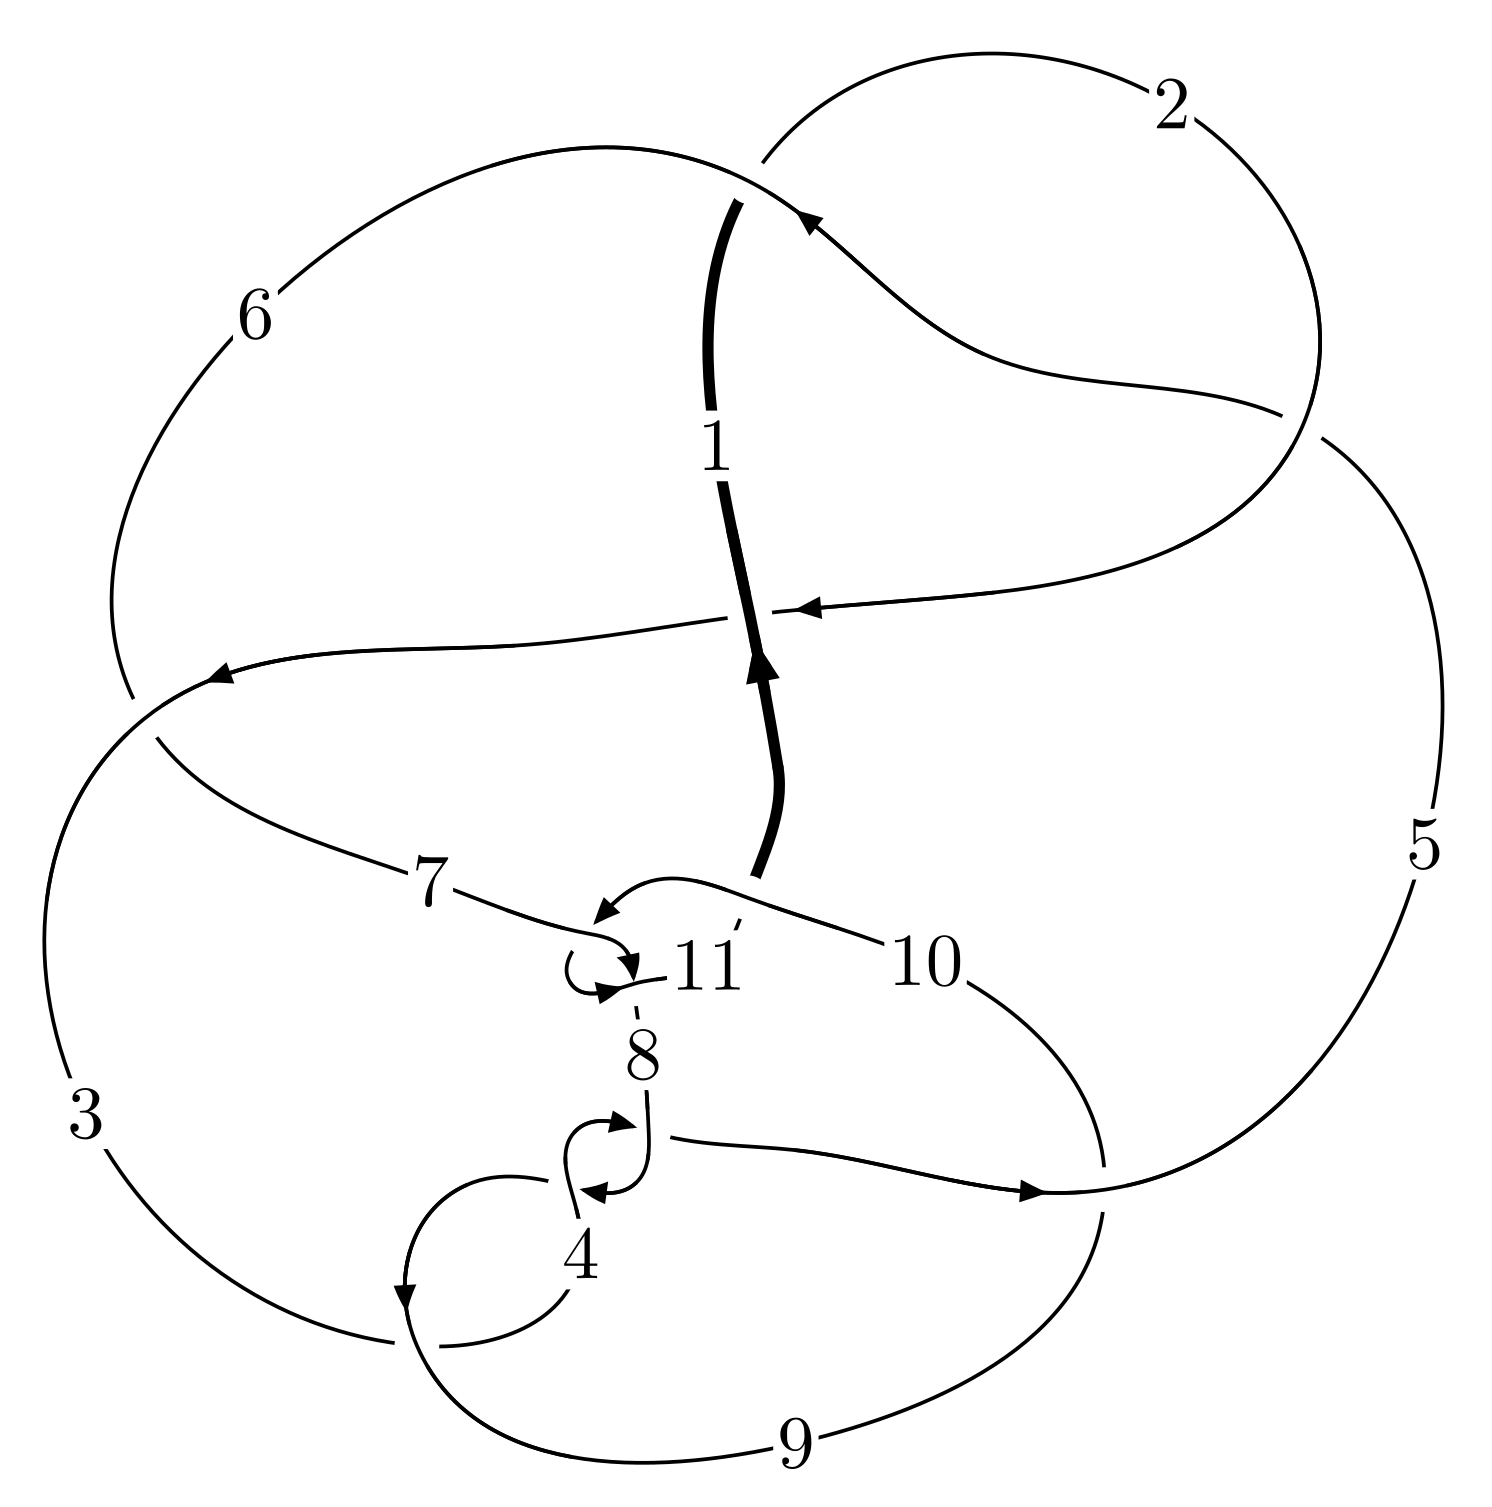
\includegraphics[width=112pt]{../../../GIT/diagram.site/Diagrams/png/336_11a_87.png}\\
\ \ \ A knot diagram\footnotemark}&
\allowdisplaybreaks
\textbf{Linearized knot diagam} \\
\cline{2-2}
 &
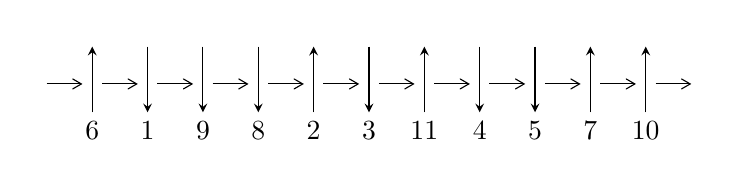
\begin{tikzpicture}[x=20pt, y=17pt]
	% nodes
	\node (C0) at (0, 0) {};
	\node (C1) at (1, 0) {};
	\node (C1U) at (1, +1) {};
	\node (C1D) at (1, -1) {6};

	\node (C2) at (2, 0) {};
	\node (C2U) at (2, +1) {};
	\node (C2D) at (2, -1) {1};

	\node (C3) at (3, 0) {};
	\node (C3U) at (3, +1) {};
	\node (C3D) at (3, -1) {9};

	\node (C4) at (4, 0) {};
	\node (C4U) at (4, +1) {};
	\node (C4D) at (4, -1) {8};

	\node (C5) at (5, 0) {};
	\node (C5U) at (5, +1) {};
	\node (C5D) at (5, -1) {2};

	\node (C6) at (6, 0) {};
	\node (C6U) at (6, +1) {};
	\node (C6D) at (6, -1) {3};

	\node (C7) at (7, 0) {};
	\node (C7U) at (7, +1) {};
	\node (C7D) at (7, -1) {11};

	\node (C8) at (8, 0) {};
	\node (C8U) at (8, +1) {};
	\node (C8D) at (8, -1) {4};

	\node (C9) at (9, 0) {};
	\node (C9U) at (9, +1) {};
	\node (C9D) at (9, -1) {5};

	\node (C10) at (10, 0) {};
	\node (C10U) at (10, +1) {};
	\node (C10D) at (10, -1) {7};

	\node (C11) at (11, 0) {};
	\node (C11U) at (11, +1) {};
	\node (C11D) at (11, -1) {10};
	\node (C12) at (12, 0) {};

	% arrows
	\draw[->,>={angle 60}]
	(C0) edge (C1) (C1) edge (C2) (C2) edge (C3) (C3) edge (C4) (C4) edge (C5) (C5) edge (C6) (C6) edge (C7) (C7) edge (C8) (C8) edge (C9) (C9) edge (C10) (C10) edge (C11) (C11) edge (C12) ;	\draw[->,>=stealth]
	(C1D) edge (C1U) (C2U) edge (C2D) (C3U) edge (C3D) (C4U) edge (C4D) (C5D) edge (C5U) (C6U) edge (C6D) (C7D) edge (C7U) (C8U) edge (C8D) (C9U) edge (C9D) (C10D) edge (C10U) (C11D) edge (C11U) ;
	\end{tikzpicture} \\
\hhline{~~} \\& 
\textbf{Solving Sequence} \\ \cline{2-2} 
 &
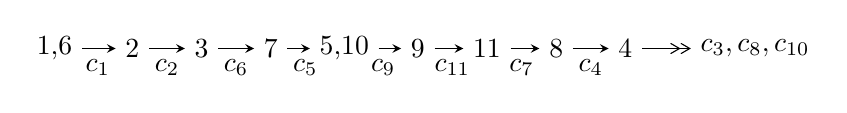
\begin{tikzpicture}[x=25pt, y=7pt]
	% node
	\node (A0) at (-1/8, 0) {1,6};
	\node (A1) at (1, 0) {2};
	\node (A2) at (2, 0) {3};
	\node (A3) at (3, 0) {7};
	\node (A4) at (65/16, 0) {5,10};
	\node (A5) at (41/8, 0) {9};
	\node (A6) at (49/8, 0) {11};
	\node (A7) at (57/8, 0) {8};
	\node (A8) at (65/8, 0) {4};
	\node (C1) at (1/2, -1) {$c_{1}$};
	\node (C2) at (3/2, -1) {$c_{2}$};
	\node (C3) at (5/2, -1) {$c_{6}$};
	\node (C4) at (7/2, -1) {$c_{5}$};
	\node (C5) at (37/8, -1) {$c_{9}$};
	\node (C6) at (45/8, -1) {$c_{11}$};
	\node (C7) at (53/8, -1) {$c_{7}$};
	\node (C8) at (61/8, -1) {$c_{4}$};
	\node (A9) at (10, 0) {$c_{3},c_{8},c_{10}$};

	% edge
	\draw[->,>=stealth]	
	(A0) edge (A1) (A1) edge (A2) (A2) edge (A3) (A3) edge (A4) (A4) edge (A5) (A5) edge (A6) (A6) edge (A7) (A7) edge (A8) ;
	\draw[->>,>={angle 60}]	
	(A8) edge (A9);
\end{tikzpicture} \\ 

\end{tabular} \\

\footnotetext{
The image of knot diagram is generated by the software ``\textbf{Draw programme}" developed by Andrew Bartholomew(\url{http://www.layer8.co.uk/maths/draw/index.htm\#Running-draw}), where we modified some parts for our purpose(\url{https://github.com/CATsTAILs/LinksPainter}).
}\phantom \\ \newline 
\centering \textbf{Ideals for irreducible components\footnotemark of $X_{\text{par}}$} 
 
\begin{align*}
I^u_{1}&=\langle 
-2.76827\times10^{20} u^{65}-3.94428\times10^{20} u^{64}+\cdots+3.38827\times10^{20} b-3.37636\times10^{20},\\
\phantom{I^u_{1}}&\phantom{= \langle  }1.46899\times10^{21} u^{65}+7.18335\times10^{20} u^{64}+\cdots+2.03296\times10^{21} a-4.01396\times10^{21},\;u^{66}+2 u^{65}+\cdots+9 u+3\rangle \\
I^u_{2}&=\langle 
b-1,\;a^2-2 a u+2 a+u-2,\;u^2- u+1\rangle \\
I^u_{3}&=\langle 
b-1,\;a+u+1,\;u^2+u+1\rangle \\
\\
\end{align*}
\raggedright * 3 irreducible components of $\dim_{\mathbb{C}}=0$, with total 72 representations.\\
\footnotetext{All coefficients of polynomials are rational numbers. But the coefficients are sometimes approximated in decimal forms when there is not enough margin.}
\newpage
\renewcommand{\arraystretch}{1}
\centering \section*{I. $I^u_{1}= \langle -2.77\times10^{20} u^{65}-3.94\times10^{20} u^{64}+\cdots+3.39\times10^{20} b-3.38\times10^{20},\;1.47\times10^{21} u^{65}+7.18\times10^{20} u^{64}+\cdots+2.03\times10^{21} a-4.01\times10^{21},\;u^{66}+2 u^{65}+\cdots+9 u+3 \rangle$}
\flushleft \textbf{(i) Arc colorings}\\
\begin{tabular}{m{7pt} m{180pt} m{7pt} m{180pt} }
\flushright $a_{1}=$&$\begin{pmatrix}1\\0\end{pmatrix}$ \\
\flushright $a_{6}=$&$\begin{pmatrix}0\\u\end{pmatrix}$ \\
\flushright $a_{2}=$&$\begin{pmatrix}1\\- u^2\end{pmatrix}$ \\
\flushright $a_{3}=$&$\begin{pmatrix}u^2+1\\- u^2\end{pmatrix}$ \\
\flushright $a_{7}=$&$\begin{pmatrix}- u^5-2 u^3- u\\u^5+u^3+u\end{pmatrix}$ \\
\flushright $a_{5}=$&$\begin{pmatrix}- u\\u^3+u\end{pmatrix}$ \\
\flushright $a_{10}=$&$\begin{pmatrix}-0.722586 u^{65}-0.353344 u^{64}+\cdots+4.62019 u+1.97444\\0.817018 u^{65}+1.16410 u^{64}+\cdots+3.14431 u+0.996486\end{pmatrix}$ \\
\flushright $a_{9}=$&$\begin{pmatrix}-0.240968 u^{65}+0.706381 u^{64}+\cdots+8.22401 u+3.27525\\0.769366 u^{65}+0.828277 u^{64}+\cdots+1.85375 u-0.0148534\end{pmatrix}$ \\
\flushright $a_{11}=$&$\begin{pmatrix}0.621466 u^{65}+1.92904 u^{64}+\cdots+12.3901 u+5.69831\\0.738277 u^{65}+0.691862 u^{64}+\cdots+0.186232 u-1.40925\end{pmatrix}$ \\
\flushright $a_{8}=$&$\begin{pmatrix}0.00495114 u^{65}+0.779268 u^{64}+\cdots+4.72824 u+1.89831\\1.18832 u^{65}+1.94777 u^{64}+\cdots+5.44396 u+0.722904\end{pmatrix}$ \\
\flushright $a_{4}=$&$\begin{pmatrix}1.01619 u^{65}+2.39037 u^{64}+\cdots+8.96868 u+4.74556\\0.357982 u^{65}-0.423891 u^{64}+\cdots-4.40018 u-3.04858\end{pmatrix}$\\ \flushright $a_{4}=$&$\begin{pmatrix}1.01619 u^{65}+2.39037 u^{64}+\cdots+8.96868 u+4.74556\\0.357982 u^{65}-0.423891 u^{64}+\cdots-4.40018 u-3.04858\end{pmatrix}$\\&\end{tabular}
\flushleft \textbf{(ii) Obstruction class $= -1$}\\~\\
\flushleft \textbf{(iii) Cusp Shapes $= \frac{637819945328403808339}{338826759075039659107} u^{65}+\frac{1108465925103697174201}{338826759075039659107} u^{64}+\cdots+\frac{3852435380313220749703}{338826759075039659107} u+\frac{473140454884407107541}{338826759075039659107}$}\\~\\
\newpage\renewcommand{\arraystretch}{1}
\flushleft \textbf{(iv) u-Polynomials at the component}\newline \\
\begin{tabular}{m{50pt}|m{274pt}}
Crossings & \hspace{64pt}u-Polynomials at each crossing \\
\hline $$\begin{aligned}c_{1},c_{5}\end{aligned}$$&$\begin{aligned}
&u^{66}-2 u^{65}+\cdots-9 u+3
\end{aligned}$\\
\hline $$\begin{aligned}c_{2}\end{aligned}$$&$\begin{aligned}
&u^{66}+32 u^{65}+\cdots+33 u+9
\end{aligned}$\\
\hline $$\begin{aligned}c_{3},c_{4},c_{8}\end{aligned}$$&$\begin{aligned}
&u^{66}+u^{65}+\cdots+16 u+4
\end{aligned}$\\
\hline $$\begin{aligned}c_{6}\end{aligned}$$&$\begin{aligned}
&u^{66}+2 u^{65}+\cdots+9195 u+2391
\end{aligned}$\\
\hline $$\begin{aligned}c_{7},c_{10}\end{aligned}$$&$\begin{aligned}
&u^{66}-3 u^{65}+\cdots-16 u+3
\end{aligned}$\\
\hline $$\begin{aligned}c_{9}\end{aligned}$$&$\begin{aligned}
&u^{66}- u^{65}+\cdots-64 u+548
\end{aligned}$\\
\hline $$\begin{aligned}c_{11}\end{aligned}$$&$\begin{aligned}
&u^{66}-33 u^{65}+\cdots-4 u+9
\end{aligned}$\\
\hline
\end{tabular}\\~\\
\newpage\renewcommand{\arraystretch}{1}
\flushleft \textbf{(v) Riley Polynomials at the component}\newline \\
\begin{tabular}{m{50pt}|m{274pt}}
Crossings & \hspace{64pt}Riley Polynomials at each crossing \\
\hline $$\begin{aligned}c_{1},c_{5}\end{aligned}$$&$\begin{aligned}
&y^{66}+32 y^{65}+\cdots+33 y+9
\end{aligned}$\\
\hline $$\begin{aligned}c_{2}\end{aligned}$$&$\begin{aligned}
&y^{66}+8 y^{65}+\cdots+873 y+81
\end{aligned}$\\
\hline $$\begin{aligned}c_{3},c_{4},c_{8}\end{aligned}$$&$\begin{aligned}
&y^{66}+61 y^{65}+\cdots-128 y+16
\end{aligned}$\\
\hline $$\begin{aligned}c_{6}\end{aligned}$$&$\begin{aligned}
&y^{66}-16 y^{65}+\cdots-60107223 y+5716881
\end{aligned}$\\
\hline $$\begin{aligned}c_{7},c_{10}\end{aligned}$$&$\begin{aligned}
&y^{66}-33 y^{65}+\cdots-4 y+9
\end{aligned}$\\
\hline $$\begin{aligned}c_{9}\end{aligned}$$&$\begin{aligned}
&y^{66}+y^{65}+\cdots-1284224 y+300304
\end{aligned}$\\
\hline $$\begin{aligned}c_{11}\end{aligned}$$&$\begin{aligned}
&y^{66}+7 y^{65}+\cdots-2176 y+81
\end{aligned}$\\
\hline
\end{tabular}\\~\\
\newpage\flushleft \textbf{(vi) Complex Volumes and Cusp Shapes}
$$\begin{array}{c|c|c}  
\text{Solutions to }I^u_{1}& \I (\text{vol} + \sqrt{-1}CS) & \text{Cusp shape}\\
 \hline 
\begin{aligned}
u &= \phantom{-}0.755953 + 0.642253 I \\
a &= -1.50344 - 0.99906 I \\
b &= \phantom{-}0.91082 + 1.08246 I\end{aligned}
 & \phantom{-}7.19005 + 6.79978 I & \phantom{-}5.09513 - 6.93835 I \\ \hline\begin{aligned}
u &= \phantom{-}0.755953 - 0.642253 I \\
a &= -1.50344 + 0.99906 I \\
b &= \phantom{-}0.91082 - 1.08246 I\end{aligned}
 & \phantom{-}7.19005 - 6.79978 I & \phantom{-}5.09513 + 6.93835 I \\ \hline\begin{aligned}
u &= \phantom{-}0.381443 + 0.962354 I \\
a &= \phantom{-}1.84405 - 1.05401 I \\
b &= \phantom{-}0.434581 - 0.385324 I\end{aligned}
 & \phantom{-}5.19371 + 1.45398 I & \phantom{-0.000000 } 0 \\ \hline\begin{aligned}
u &= \phantom{-}0.381443 - 0.962354 I \\
a &= \phantom{-}1.84405 + 1.05401 I \\
b &= \phantom{-}0.434581 + 0.385324 I\end{aligned}
 & \phantom{-}5.19371 - 1.45398 I & \phantom{-0.000000 } 0 \\ \hline\begin{aligned}
u &= -0.673098 + 0.678865 I \\
a &= -1.193220 + 0.537398 I \\
b &= \phantom{-}0.813918 - 0.796640 I\end{aligned}
 & \phantom{-}1.97562 - 3.83931 I & \phantom{-}0.43158 + 7.99484 I \\ \hline\begin{aligned}
u &= -0.673098 - 0.678865 I \\
a &= -1.193220 - 0.537398 I \\
b &= \phantom{-}0.813918 + 0.796640 I\end{aligned}
 & \phantom{-}1.97562 + 3.83931 I & \phantom{-}0.43158 - 7.99484 I \\ \hline\begin{aligned}
u &= \phantom{-}0.638302 + 0.703727 I \\
a &= \phantom{-}1.149350 + 0.463060 I \\
b &= -0.200847 - 0.267724 I\end{aligned}
 & \phantom{-}4.99477 + 2.60395 I & \phantom{-}2.08066 - 2.86296 I \\ \hline\begin{aligned}
u &= \phantom{-}0.638302 - 0.703727 I \\
a &= \phantom{-}1.149350 - 0.463060 I \\
b &= -0.200847 + 0.267724 I\end{aligned}
 & \phantom{-}4.99477 - 2.60395 I & \phantom{-}2.08066 + 2.86296 I \\ \hline\begin{aligned}
u &= -0.316058 + 1.015530 I \\
a &= -0.80720 - 1.18230 I \\
b &= \phantom{-}1.59297 - 0.23810 I\end{aligned}
 & \phantom{-}4.37513 - 0.91344 I & \phantom{-0.000000 } 0 \\ \hline\begin{aligned}
u &= -0.316058 - 1.015530 I \\
a &= -0.80720 + 1.18230 I \\
b &= \phantom{-}1.59297 + 0.23810 I\end{aligned}
 & \phantom{-}4.37513 + 0.91344 I & \phantom{-0.000000 } 0\\
 \hline 
 \end{array}$$\newpage$$\begin{array}{c|c|c}  
\text{Solutions to }I^u_{1}& \I (\text{vol} + \sqrt{-1}CS) & \text{Cusp shape}\\
 \hline 
\begin{aligned}
u &= \phantom{-}0.629972 + 0.864578 I \\
a &= \phantom{-}0.282045 - 0.437369 I \\
b &= \phantom{-}0.105832 + 0.332549 I\end{aligned}
 & \phantom{-}4.56888 + 2.29703 I & \phantom{-0.000000 } 0 \\ \hline\begin{aligned}
u &= \phantom{-}0.629972 - 0.864578 I \\
a &= \phantom{-}0.282045 + 0.437369 I \\
b &= \phantom{-}0.105832 - 0.332549 I\end{aligned}
 & \phantom{-}4.56888 - 2.29703 I & \phantom{-0.000000 } 0 \\ \hline\begin{aligned}
u &= -0.827182 + 0.359098 I \\
a &= -1.48252 - 1.13505 I \\
b &= \phantom{-}1.00026 + 1.36192 I\end{aligned}
 & \phantom{-}5.59217 + 9.84151 I & \phantom{-}4.35993 - 5.90567 I \\ \hline\begin{aligned}
u &= -0.827182 - 0.359098 I \\
a &= -1.48252 + 1.13505 I \\
b &= \phantom{-}1.00026 - 1.36192 I\end{aligned}
 & \phantom{-}5.59217 - 9.84151 I & \phantom{-}4.35993 + 5.90567 I \\ \hline\begin{aligned}
u &= -0.615669 + 0.911613 I \\
a &= \phantom{-}0.149118 - 1.152950 I \\
b &= \phantom{-}0.719356 + 0.533955 I\end{aligned}
 & \phantom{-}1.29731 - 1.14051 I & \phantom{-0.000000 } 0 \\ \hline\begin{aligned}
u &= -0.615669 - 0.911613 I \\
a &= \phantom{-}0.149118 + 1.152950 I \\
b &= \phantom{-}0.719356 - 0.533955 I\end{aligned}
 & \phantom{-}1.29731 + 1.14051 I & \phantom{-0.000000 } 0 \\ \hline\begin{aligned}
u &= \phantom{-}0.484610 + 1.022030 I \\
a &= -0.59263 + 1.37966 I \\
b &= \phantom{-}1.48883 - 0.30554 I\end{aligned}
 & \phantom{-}1.07785 + 3.02843 I & \phantom{-0.000000 } 0 \\ \hline\begin{aligned}
u &= \phantom{-}0.484610 - 1.022030 I \\
a &= -0.59263 - 1.37966 I \\
b &= \phantom{-}1.48883 + 0.30554 I\end{aligned}
 & \phantom{-}1.07785 - 3.02843 I & \phantom{-0.000000 } 0 \\ \hline\begin{aligned}
u &= \phantom{-}0.789237 + 0.311182 I \\
a &= -1.14249 + 0.91939 I \\
b &= \phantom{-}0.83658 - 1.26862 I\end{aligned}
 & \phantom{-}0.08192 - 6.09483 I & \phantom{-}0.06758 + 5.72110 I \\ \hline\begin{aligned}
u &= \phantom{-}0.789237 - 0.311182 I \\
a &= -1.14249 - 0.91939 I \\
b &= \phantom{-}0.83658 + 1.26862 I\end{aligned}
 & \phantom{-}0.08192 + 6.09483 I & \phantom{-}0.06758 - 5.72110 I\\
 \hline 
 \end{array}$$\newpage$$\begin{array}{c|c|c}  
\text{Solutions to }I^u_{1}& \I (\text{vol} + \sqrt{-1}CS) & \text{Cusp shape}\\
 \hline 
\begin{aligned}
u &= -0.772578 + 0.300651 I \\
a &= \phantom{-}1.43595 + 0.47376 I \\
b &= -0.606077 - 0.508848 I\end{aligned}
 & \phantom{-}3.05327 + 4.56939 I & \phantom{-}1.49874 - 2.48258 I \\ \hline\begin{aligned}
u &= -0.772578 - 0.300651 I \\
a &= \phantom{-}1.43595 - 0.47376 I \\
b &= -0.606077 + 0.508848 I\end{aligned}
 & \phantom{-}3.05327 - 4.56939 I & \phantom{-}1.49874 + 2.48258 I \\ \hline\begin{aligned}
u &= -0.327983 + 1.126830 I \\
a &= \phantom{-}0.973843 + 0.583016 I \\
b &= \phantom{-}0.256425 + 1.074870 I\end{aligned}
 & -2.37023 - 1.02641 I & \phantom{-0.000000 } 0 \\ \hline\begin{aligned}
u &= -0.327983 - 1.126830 I \\
a &= \phantom{-}0.973843 - 0.583016 I \\
b &= \phantom{-}0.256425 - 1.074870 I\end{aligned}
 & -2.37023 + 1.02641 I & \phantom{-0.000000 } 0 \\ \hline\begin{aligned}
u &= \phantom{-}0.666510 + 0.972232 I \\
a &= \phantom{-}0.23112 + 1.62158 I \\
b &= \phantom{-}0.834491 - 0.957996 I\end{aligned}
 & \phantom{-}6.21106 - 1.42535 I & \phantom{-0.000000 } 0 \\ \hline\begin{aligned}
u &= \phantom{-}0.666510 - 0.972232 I \\
a &= \phantom{-}0.23112 - 1.62158 I \\
b &= \phantom{-}0.834491 + 0.957996 I\end{aligned}
 & \phantom{-}6.21106 + 1.42535 I & \phantom{-0.000000 } 0 \\ \hline\begin{aligned}
u &= -0.254618 + 1.152190 I \\
a &= \phantom{-}0.308382 - 0.112718 I \\
b &= -0.492338 - 0.741909 I\end{aligned}
 & -1.45645 + 1.57837 I & \phantom{-0.000000 } 0 \\ \hline\begin{aligned}
u &= -0.254618 - 1.152190 I \\
a &= \phantom{-}0.308382 + 0.112718 I \\
b &= -0.492338 + 0.741909 I\end{aligned}
 & -1.45645 - 1.57837 I & \phantom{-0.000000 } 0 \\ \hline\begin{aligned}
u &= \phantom{-}0.530812 + 1.055770 I \\
a &= -1.34138 + 2.03995 I \\
b &= \phantom{-}0.816422 + 0.889494 I\end{aligned}
 & \phantom{-}6.42459 + 4.74081 I & \phantom{-0.000000 } 0 \\ \hline\begin{aligned}
u &= \phantom{-}0.530812 - 1.055770 I \\
a &= -1.34138 - 2.03995 I \\
b &= \phantom{-}0.816422 - 0.889494 I\end{aligned}
 & \phantom{-}6.42459 - 4.74081 I & \phantom{-0.000000 } 0\\
 \hline 
 \end{array}$$\newpage$$\begin{array}{c|c|c}  
\text{Solutions to }I^u_{1}& \I (\text{vol} + \sqrt{-1}CS) & \text{Cusp shape}\\
 \hline 
\begin{aligned}
u &= \phantom{-}0.241965 + 1.161020 I \\
a &= \phantom{-}0.593783 - 0.497940 I \\
b &= \phantom{-}0.56461 - 1.30292 I\end{aligned}
 & -4.56064 - 3.10867 I & \phantom{-0.000000 } 0 \\ \hline\begin{aligned}
u &= \phantom{-}0.241965 - 1.161020 I \\
a &= \phantom{-}0.593783 + 0.497940 I \\
b &= \phantom{-}0.56461 + 1.30292 I\end{aligned}
 & -4.56064 + 3.10867 I & \phantom{-0.000000 } 0 \\ \hline\begin{aligned}
u &= -0.179712 + 1.178530 I \\
a &= \phantom{-}0.312033 + 0.454932 I \\
b &= \phantom{-}0.80836 + 1.39012 I\end{aligned}
 & \phantom{-}0.48993 + 7.02185 I & \phantom{-0.000000 } 0 \\ \hline\begin{aligned}
u &= -0.179712 - 1.178530 I \\
a &= \phantom{-}0.312033 - 0.454932 I \\
b &= \phantom{-}0.80836 - 1.39012 I\end{aligned}
 & \phantom{-}0.48993 - 7.02185 I & \phantom{-0.000000 } 0 \\ \hline\begin{aligned}
u &= \phantom{-}0.337552 + 1.150340 I \\
a &= \phantom{-}0.029903 + 0.280018 I \\
b &= -0.229833 + 0.947989 I\end{aligned}
 & -5.71596 + 2.27676 I & \phantom{-0.000000 } 0 \\ \hline\begin{aligned}
u &= \phantom{-}0.337552 - 1.150340 I \\
a &= \phantom{-}0.029903 - 0.280018 I \\
b &= -0.229833 - 0.947989 I\end{aligned}
 & -5.71596 - 2.27676 I & \phantom{-0.000000 } 0 \\ \hline\begin{aligned}
u &= -0.441361 + 1.120500 I \\
a &= \phantom{-}1.302260 + 0.531091 I \\
b &= -0.196410 + 0.826154 I\end{aligned}
 & -2.36959 - 1.62048 I & \phantom{-0.000000 } 0 \\ \hline\begin{aligned}
u &= -0.441361 - 1.120500 I \\
a &= \phantom{-}1.302260 - 0.531091 I \\
b &= -0.196410 - 0.826154 I\end{aligned}
 & -2.36959 + 1.62048 I & \phantom{-0.000000 } 0 \\ \hline\begin{aligned}
u &= -0.539438 + 1.080200 I \\
a &= -0.58267 - 1.65912 I \\
b &= \phantom{-}1.64758 + 0.62868 I\end{aligned}
 & \phantom{-}5.95344 - 5.84050 I & \phantom{-0.000000 } 0 \\ \hline\begin{aligned}
u &= -0.539438 - 1.080200 I \\
a &= -0.58267 + 1.65912 I \\
b &= \phantom{-}1.64758 - 0.62868 I\end{aligned}
 & \phantom{-}5.95344 + 5.84050 I & \phantom{-0.000000 } 0\\
 \hline 
 \end{array}$$\newpage$$\begin{array}{c|c|c}  
\text{Solutions to }I^u_{1}& \I (\text{vol} + \sqrt{-1}CS) & \text{Cusp shape}\\
 \hline 
\begin{aligned}
u &= -0.416062 + 1.153030 I \\
a &= -0.417211 - 0.486945 I \\
b &= \phantom{-}0.078553 - 1.146340 I\end{aligned}
 & -2.51166 - 6.30368 I & \phantom{-0.000000 } 0 \\ \hline\begin{aligned}
u &= -0.416062 - 1.153030 I \\
a &= -0.417211 + 0.486945 I \\
b &= \phantom{-}0.078553 + 1.146340 I\end{aligned}
 & -2.51166 + 6.30368 I & \phantom{-0.000000 } 0 \\ \hline\begin{aligned}
u &= -0.529988 + 1.122110 I \\
a &= -1.43472 - 1.07430 I \\
b &= \phantom{-}0.70216 - 1.23357 I\end{aligned}
 & -0.97780 - 6.67256 I & \phantom{-0.000000 } 0 \\ \hline\begin{aligned}
u &= -0.529988 - 1.122110 I \\
a &= -1.43472 + 1.07430 I \\
b &= \phantom{-}0.70216 + 1.23357 I\end{aligned}
 & -0.97780 + 6.67256 I & \phantom{-0.000000 } 0 \\ \hline\begin{aligned}
u &= \phantom{-}0.515018 + 1.137380 I \\
a &= \phantom{-}1.42983 - 0.56620 I \\
b &= -0.550564 - 0.698729 I\end{aligned}
 & -4.51086 + 5.70416 I & \phantom{-0.000000 } 0 \\ \hline\begin{aligned}
u &= \phantom{-}0.515018 - 1.137380 I \\
a &= \phantom{-}1.42983 + 0.56620 I \\
b &= -0.550564 + 0.698729 I\end{aligned}
 & -4.51086 - 5.70416 I & \phantom{-0.000000 } 0 \\ \hline\begin{aligned}
u &= \phantom{-}0.595919 + 0.445110 I \\
a &= -1.71034 - 0.58122 I \\
b &= \phantom{-}1.032560 - 0.749088 I\end{aligned}
 & \phantom{-}8.21032 - 0.24162 I & \phantom{-}6.87319 + 1.62100 I \\ \hline\begin{aligned}
u &= \phantom{-}0.595919 - 0.445110 I \\
a &= -1.71034 + 0.58122 I \\
b &= \phantom{-}1.032560 + 0.749088 I\end{aligned}
 & \phantom{-}8.21032 + 0.24162 I & \phantom{-}6.87319 - 1.62100 I \\ \hline\begin{aligned}
u &= -0.634539 + 0.386396 I \\
a &= -2.62691 + 0.09834 I \\
b &= \phantom{-}1.45210 - 0.62541 I\end{aligned}
 & \phantom{-}7.96080 + 1.22074 I & \phantom{-}6.79923 - 0.85488 I \\ \hline\begin{aligned}
u &= -0.634539 - 0.386396 I \\
a &= -2.62691 - 0.09834 I \\
b &= \phantom{-}1.45210 + 0.62541 I\end{aligned}
 & \phantom{-}7.96080 - 1.22074 I & \phantom{-}6.79923 + 0.85488 I\\
 \hline 
 \end{array}$$\newpage$$\begin{array}{c|c|c}  
\text{Solutions to }I^u_{1}& \I (\text{vol} + \sqrt{-1}CS) & \text{Cusp shape}\\
 \hline 
\begin{aligned}
u &= \phantom{-}0.495446 + 0.549605 I \\
a &= -1.81945 + 0.43460 I \\
b &= \phantom{-}1.158230 + 0.508717 I\end{aligned}
 & \phantom{-}2.51441 + 1.02533 I & \phantom{-}3.07736 + 2.06010 I \\ \hline\begin{aligned}
u &= \phantom{-}0.495446 - 0.549605 I \\
a &= -1.81945 - 0.43460 I \\
b &= \phantom{-}1.158230 - 0.508717 I\end{aligned}
 & \phantom{-}2.51441 - 1.02533 I & \phantom{-}3.07736 - 2.06010 I \\ \hline\begin{aligned}
u &= -0.279936 + 0.676376 I \\
a &= \phantom{-}0.982603 - 0.117408 I \\
b &= -0.148031 - 0.060354 I\end{aligned}
 & -0.280767 - 1.133580 I & -3.39541 + 6.11783 I \\ \hline\begin{aligned}
u &= -0.279936 - 0.676376 I \\
a &= \phantom{-}0.982603 + 0.117408 I \\
b &= -0.148031 + 0.060354 I\end{aligned}
 & -0.280767 + 1.133580 I & -3.39541 - 6.11783 I \\ \hline\begin{aligned}
u &= -0.560271 + 1.138380 I \\
a &= \phantom{-}1.48877 + 0.66169 I \\
b &= -0.742454 + 0.556217 I\end{aligned}
 & \phantom{-}0.59224 - 9.57146 I & \phantom{-0.000000 } 0 \\ \hline\begin{aligned}
u &= -0.560271 - 1.138380 I \\
a &= \phantom{-}1.48877 - 0.66169 I \\
b &= -0.742454 - 0.556217 I\end{aligned}
 & \phantom{-}0.59224 + 9.57146 I & \phantom{-0.000000 } 0 \\ \hline\begin{aligned}
u &= \phantom{-}0.702291 + 0.195645 I \\
a &= \phantom{-}1.088270 - 0.495569 I \\
b &= -0.323516 + 0.616413 I\end{aligned}
 & -1.84194 - 1.10470 I & -3.59487 + 1.11336 I \\ \hline\begin{aligned}
u &= \phantom{-}0.702291 - 0.195645 I \\
a &= \phantom{-}1.088270 + 0.495569 I \\
b &= -0.323516 - 0.616413 I\end{aligned}
 & -1.84194 + 1.10470 I & -3.59487 - 1.11336 I \\ \hline\begin{aligned}
u &= -0.673885 + 0.269171 I \\
a &= -0.765242 - 0.266085 I \\
b &= \phantom{-}0.709105 + 0.972863 I\end{aligned}
 & \phantom{-}1.45545 + 2.02266 I & \phantom{-}2.54801 - 0.95165 I \\ \hline\begin{aligned}
u &= -0.673885 - 0.269171 I \\
a &= -0.765242 + 0.266085 I \\
b &= \phantom{-}0.709105 - 0.972863 I\end{aligned}
 & \phantom{-}1.45545 - 2.02266 I & \phantom{-}2.54801 + 0.95165 I\\
 \hline 
 \end{array}$$\newpage$$\begin{array}{c|c|c}  
\text{Solutions to }I^u_{1}& \I (\text{vol} + \sqrt{-1}CS) & \text{Cusp shape}\\
 \hline 
\begin{aligned}
u &= \phantom{-}0.568245 + 1.141590 I \\
a &= -1.88642 + 0.84516 I \\
b &= \phantom{-}0.87554 + 1.41049 I\end{aligned}
 & -2.37082 + 11.17440 I & \phantom{-0.000000 } 0 \\ \hline\begin{aligned}
u &= \phantom{-}0.568245 - 1.141590 I \\
a &= -1.88642 - 0.84516 I \\
b &= \phantom{-}0.87554 - 1.41049 I\end{aligned}
 & -2.37082 - 11.17440 I & \phantom{-0.000000 } 0 \\ \hline\begin{aligned}
u &= -0.596220 + 1.140020 I \\
a &= -2.20616 - 0.82618 I \\
b &= \phantom{-}1.03862 - 1.45053 I\end{aligned}
 & \phantom{-}3.2588 - 15.1381 I & \phantom{-0.000000 } 0 \\ \hline\begin{aligned}
u &= -0.596220 - 1.140020 I \\
a &= -2.20616 + 0.82618 I \\
b &= \phantom{-}1.03862 + 1.45053 I\end{aligned}
 & \phantom{-}3.2588 + 15.1381 I & \phantom{-0.000000 } 0 \\ \hline\begin{aligned}
u &= -0.694677 + 0.021213 I \\
a &= \phantom{-}0.410694 - 0.577612 I \\
b &= \phantom{-}0.112167 + 0.890796 I\end{aligned}
 & \phantom{-}0.77779 + 2.28714 I & \phantom{-}0.68771 - 3.78757 I \\ \hline\begin{aligned}
u &= -0.694677 - 0.021213 I \\
a &= \phantom{-}0.410694 + 0.577612 I \\
b &= \phantom{-}0.112167 - 0.890796 I\end{aligned}
 & \phantom{-}0.77779 - 2.28714 I & \phantom{-}0.68771 + 3.78757 I\\
 \hline 
 \end{array}$$\newpage\newpage\renewcommand{\arraystretch}{1}
\centering \section*{II. $I^u_{2}= \langle b-1,\;a^2-2 a u+2 a+u-2,\;u^2- u+1 \rangle$}
\flushleft \textbf{(i) Arc colorings}\\
\begin{tabular}{m{7pt} m{180pt} m{7pt} m{180pt} }
\flushright $a_{1}=$&$\begin{pmatrix}1\\0\end{pmatrix}$ \\
\flushright $a_{6}=$&$\begin{pmatrix}0\\u\end{pmatrix}$ \\
\flushright $a_{2}=$&$\begin{pmatrix}1\\- u+1\end{pmatrix}$ \\
\flushright $a_{3}=$&$\begin{pmatrix}u\\- u+1\end{pmatrix}$ \\
\flushright $a_{7}=$&$\begin{pmatrix}1\\0\end{pmatrix}$ \\
\flushright $a_{5}=$&$\begin{pmatrix}- u\\u-1\end{pmatrix}$ \\
\flushright $a_{10}=$&$\begin{pmatrix}a\\1\end{pmatrix}$ \\
\flushright $a_{9}=$&$\begin{pmatrix}u-1\\a u+2\end{pmatrix}$ \\
\flushright $a_{11}=$&$\begin{pmatrix}a+1\\1\end{pmatrix}$ \\
\flushright $a_{8}=$&$\begin{pmatrix}- a\\-1\end{pmatrix}$ \\
\flushright $a_{4}=$&$\begin{pmatrix}- a u+u-1\\a u- a+2 u-1\end{pmatrix}$\\ \flushright $a_{4}=$&$\begin{pmatrix}- a u+u-1\\a u- a+2 u-1\end{pmatrix}$\\&\end{tabular}
\flushleft \textbf{(ii) Obstruction class $= 1$}\\~\\
\flushleft \textbf{(iii) Cusp Shapes $= -4 u+8$}\\~\\
\newpage\renewcommand{\arraystretch}{1}
\flushleft \textbf{(iv) u-Polynomials at the component}\newline \\
\begin{tabular}{m{50pt}|m{274pt}}
Crossings & \hspace{64pt}u-Polynomials at each crossing \\
\hline $$\begin{aligned}c_{1},c_{6}\end{aligned}$$&$\begin{aligned}
&(u^2- u+1)^2
\end{aligned}$\\
\hline $$\begin{aligned}c_{2},c_{5}\end{aligned}$$&$\begin{aligned}
&(u^2+u+1)^2
\end{aligned}$\\
\hline $$\begin{aligned}c_{3},c_{4},c_{8}\\c_{9}\end{aligned}$$&$\begin{aligned}
&(u^2+2)^2
\end{aligned}$\\
\hline $$\begin{aligned}c_{7},c_{11}\end{aligned}$$&$\begin{aligned}
&(u-1)^4
\end{aligned}$\\
\hline $$\begin{aligned}c_{10}\end{aligned}$$&$\begin{aligned}
&(u+1)^4
\end{aligned}$\\
\hline
\end{tabular}\\~\\
\newpage\renewcommand{\arraystretch}{1}
\flushleft \textbf{(v) Riley Polynomials at the component}\newline \\
\begin{tabular}{m{50pt}|m{274pt}}
Crossings & \hspace{64pt}Riley Polynomials at each crossing \\
\hline $$\begin{aligned}c_{1},c_{2},c_{5}\\c_{6}\end{aligned}$$&$\begin{aligned}
&(y^2+y+1)^2
\end{aligned}$\\
\hline $$\begin{aligned}c_{3},c_{4},c_{8}\\c_{9}\end{aligned}$$&$\begin{aligned}
&(y+2)^4
\end{aligned}$\\
\hline $$\begin{aligned}c_{7},c_{10},c_{11}\end{aligned}$$&$\begin{aligned}
&(y-1)^4
\end{aligned}$\\
\hline
\end{tabular}\\~\\
\newpage\flushleft \textbf{(vi) Complex Volumes and Cusp Shapes}
$$\begin{array}{c|c|c}  
\text{Solutions to }I^u_{2}& \I (\text{vol} + \sqrt{-1}CS) & \text{Cusp shape}\\
 \hline 
\begin{aligned}
u &= \phantom{-}0.500000 + 0.866025 I \\
a &= \phantom{-}0.724745 + 0.158919 I \\
b &= \phantom{-}1.00000\phantom{ +0.000000I}\end{aligned}
 & \phantom{-}6.57974 + 2.02988 I & \phantom{-}6.00000 - 3.46410 I \\ \hline\begin{aligned}
u &= \phantom{-}0.500000 + 0.866025 I \\
a &= -1.72474 + 1.57313 I \\
b &= \phantom{-}1.00000\phantom{ +0.000000I}\end{aligned}
 & \phantom{-}6.57974 + 2.02988 I & \phantom{-}6.00000 - 3.46410 I \\ \hline\begin{aligned}
u &= \phantom{-}0.500000 - 0.866025 I \\
a &= \phantom{-}0.724745 - 0.158919 I \\
b &= \phantom{-}1.00000\phantom{ +0.000000I}\end{aligned}
 & \phantom{-}6.57974 - 2.02988 I & \phantom{-}6.00000 + 3.46410 I \\ \hline\begin{aligned}
u &= \phantom{-}0.500000 - 0.866025 I \\
a &= -1.72474 - 1.57313 I \\
b &= \phantom{-}1.00000\phantom{ +0.000000I}\end{aligned}
 & \phantom{-}6.57974 - 2.02988 I & \phantom{-}6.00000 + 3.46410 I\\
 \hline 
 \end{array}$$\newpage\newpage\renewcommand{\arraystretch}{1}
\centering \section*{III. $I^u_{3}= \langle b-1,\;a+u+1,\;u^2+u+1 \rangle$}
\flushleft \textbf{(i) Arc colorings}\\
\begin{tabular}{m{7pt} m{180pt} m{7pt} m{180pt} }
\flushright $a_{1}=$&$\begin{pmatrix}1\\0\end{pmatrix}$ \\
\flushright $a_{6}=$&$\begin{pmatrix}0\\u\end{pmatrix}$ \\
\flushright $a_{2}=$&$\begin{pmatrix}1\\u+1\end{pmatrix}$ \\
\flushright $a_{3}=$&$\begin{pmatrix}- u\\u+1\end{pmatrix}$ \\
\flushright $a_{7}=$&$\begin{pmatrix}-1\\0\end{pmatrix}$ \\
\flushright $a_{5}=$&$\begin{pmatrix}- u\\u+1\end{pmatrix}$ \\
\flushright $a_{10}=$&$\begin{pmatrix}- u-1\\1\end{pmatrix}$ \\
\flushright $a_{9}=$&$\begin{pmatrix}- u-1\\1\end{pmatrix}$ \\
\flushright $a_{11}=$&$\begin{pmatrix}- u\\1\end{pmatrix}$ \\
\flushright $a_{8}=$&$\begin{pmatrix}- u-1\\1\end{pmatrix}$ \\
\flushright $a_{4}=$&$\begin{pmatrix}- u\\u+1\end{pmatrix}$\\ \flushright $a_{4}=$&$\begin{pmatrix}- u\\u+1\end{pmatrix}$\\&\end{tabular}
\flushleft \textbf{(ii) Obstruction class $= 1$}\\~\\
\flushleft \textbf{(iii) Cusp Shapes $= 4 u+2$}\\~\\
\newpage\renewcommand{\arraystretch}{1}
\flushleft \textbf{(iv) u-Polynomials at the component}\newline \\
\begin{tabular}{m{50pt}|m{274pt}}
Crossings & \hspace{64pt}u-Polynomials at each crossing \\
\hline $$\begin{aligned}c_{1},c_{2},c_{6}\end{aligned}$$&$\begin{aligned}
&u^2+u+1
\end{aligned}$\\
\hline $$\begin{aligned}c_{3},c_{4},c_{8}\\c_{9}\end{aligned}$$&$\begin{aligned}
&u^2
\end{aligned}$\\
\hline $$\begin{aligned}c_{5}\end{aligned}$$&$\begin{aligned}
&u^2- u+1
\end{aligned}$\\
\hline $$\begin{aligned}c_{7}\end{aligned}$$&$\begin{aligned}
&(u+1)^2
\end{aligned}$\\
\hline $$\begin{aligned}c_{10},c_{11}\end{aligned}$$&$\begin{aligned}
&(u-1)^2
\end{aligned}$\\
\hline
\end{tabular}\\~\\
\newpage\renewcommand{\arraystretch}{1}
\flushleft \textbf{(v) Riley Polynomials at the component}\newline \\
\begin{tabular}{m{50pt}|m{274pt}}
Crossings & \hspace{64pt}Riley Polynomials at each crossing \\
\hline $$\begin{aligned}c_{1},c_{2},c_{5}\\c_{6}\end{aligned}$$&$\begin{aligned}
&y^2+y+1
\end{aligned}$\\
\hline $$\begin{aligned}c_{3},c_{4},c_{8}\\c_{9}\end{aligned}$$&$\begin{aligned}
&y^2
\end{aligned}$\\
\hline $$\begin{aligned}c_{7},c_{10},c_{11}\end{aligned}$$&$\begin{aligned}
&(y-1)^2
\end{aligned}$\\
\hline
\end{tabular}\\~\\
\newpage\flushleft \textbf{(vi) Complex Volumes and Cusp Shapes}
$$\begin{array}{c|c|c}  
\text{Solutions to }I^u_{3}& \I (\text{vol} + \sqrt{-1}CS) & \text{Cusp shape}\\
 \hline 
\begin{aligned}
u &= -0.500000 + 0.866025 I \\
a &= -0.500000 - 0.866025 I \\
b &= \phantom{-}1.00000\phantom{ +0.000000I}\end{aligned}
 & \phantom{-}1.64493 - 2.02988 I & \phantom{-0.000000 -}0. + 3.46410 I \\ \hline\begin{aligned}
u &= -0.500000 - 0.866025 I \\
a &= -0.500000 + 0.866025 I \\
b &= \phantom{-}1.00000\phantom{ +0.000000I}\end{aligned}
 & \phantom{-}1.64493 + 2.02988 I & \phantom{-0.000000 } 0. - 3.46410 I\\
 \hline 
 \end{array}$$\newpage
\newpage\renewcommand{\arraystretch}{1}
\centering \section*{ IV. u-Polynomials}
\begin{tabular}{m{50pt}|m{274pt}}
Crossings & \hspace{64pt}u-Polynomials at each crossing \\
\hline $$\begin{aligned}c_{1}\end{aligned}$$&$\begin{aligned}
&((u^2- u+1)^2)(u^2+u+1)(u^{66}-2 u^{65}+\cdots-9 u+3)
\end{aligned}$\\
\hline $$\begin{aligned}c_{2}\end{aligned}$$&$\begin{aligned}
&((u^2+u+1)^3)(u^{66}+32 u^{65}+\cdots+33 u+9)
\end{aligned}$\\
\hline $$\begin{aligned}c_{3},c_{4},c_{8}\end{aligned}$$&$\begin{aligned}
&u^2(u^2+2)^2(u^{66}+u^{65}+\cdots+16 u+4)
\end{aligned}$\\
\hline $$\begin{aligned}c_{5}\end{aligned}$$&$\begin{aligned}
&(u^2- u+1)(u^2+u+1)^2(u^{66}-2 u^{65}+\cdots-9 u+3)
\end{aligned}$\\
\hline $$\begin{aligned}c_{6}\end{aligned}$$&$\begin{aligned}
&((u^2- u+1)^2)(u^2+u+1)(u^{66}+2 u^{65}+\cdots+9195 u+2391)
\end{aligned}$\\
\hline $$\begin{aligned}c_{7}\end{aligned}$$&$\begin{aligned}
&((u-1)^4)(u+1)^2(u^{66}-3 u^{65}+\cdots-16 u+3)
\end{aligned}$\\
\hline $$\begin{aligned}c_{9}\end{aligned}$$&$\begin{aligned}
&u^2(u^2+2)^2(u^{66}- u^{65}+\cdots-64 u+548)
\end{aligned}$\\
\hline $$\begin{aligned}c_{10}\end{aligned}$$&$\begin{aligned}
&((u-1)^2)(u+1)^4(u^{66}-3 u^{65}+\cdots-16 u+3)
\end{aligned}$\\
\hline $$\begin{aligned}c_{11}\end{aligned}$$&$\begin{aligned}
&((u-1)^6)(u^{66}-33 u^{65}+\cdots-4 u+9)
\end{aligned}$\\
\hline
\end{tabular}\newpage\renewcommand{\arraystretch}{1}
\centering \section*{ V. Riley Polynomials}
\begin{tabular}{m{50pt}|m{274pt}}
Crossings & \hspace{64pt}Riley Polynomials at each crossing \\
\hline $$\begin{aligned}c_{1},c_{5}\end{aligned}$$&$\begin{aligned}
&((y^2+y+1)^3)(y^{66}+32 y^{65}+\cdots+33 y+9)
\end{aligned}$\\
\hline $$\begin{aligned}c_{2}\end{aligned}$$&$\begin{aligned}
&((y^2+y+1)^3)(y^{66}+8 y^{65}+\cdots+873 y+81)
\end{aligned}$\\
\hline $$\begin{aligned}c_{3},c_{4},c_{8}\end{aligned}$$&$\begin{aligned}
&y^2(y+2)^4(y^{66}+61 y^{65}+\cdots-128 y+16)
\end{aligned}$\\
\hline $$\begin{aligned}c_{6}\end{aligned}$$&$\begin{aligned}
&((y^2+y+1)^3)(y^{66}-16 y^{65}+\cdots-6.01072\times10^{7} y+5716881)
\end{aligned}$\\
\hline $$\begin{aligned}c_{7},c_{10}\end{aligned}$$&$\begin{aligned}
&((y-1)^6)(y^{66}-33 y^{65}+\cdots-4 y+9)
\end{aligned}$\\
\hline $$\begin{aligned}c_{9}\end{aligned}$$&$\begin{aligned}
&y^2(y+2)^4(y^{66}+y^{65}+\cdots-1284224 y+300304)
\end{aligned}$\\
\hline $$\begin{aligned}c_{11}\end{aligned}$$&$\begin{aligned}
&((y-1)^6)(y^{66}+7 y^{65}+\cdots-2176 y+81)
\end{aligned}$\\
\hline
\end{tabular}
\vskip 2pc
\end{document}